\begin{figure}[htbp]
\centering
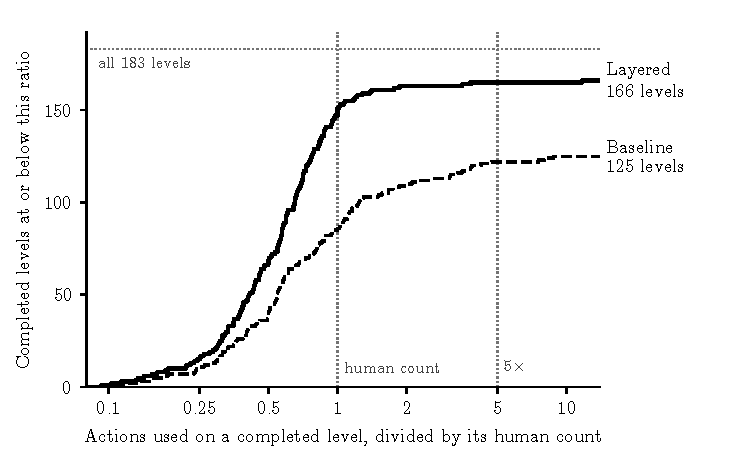
\includegraphics[width=0.74\linewidth]{figures/level_action_ratio.pdf}
\caption{\textbf{Both harnesses solved most of their completed levels within the human action count, and few levels took more than five times that count.} The horizontal axis shows the actions used to complete a level as a multiple of that level's human baseline: 1 means the same number of actions, and 5 means five times as many. The axis uses a logarithmic scale. At each point, a curve shows how many levels a harness completed using no more than that multiple. The solid curve shows the layered runs (166 completed levels), and the dashed curve shows the baseline (125). The vertical dotted lines mark 1 and 5; five times the human count is the official leaderboard's action budget for each level \citep{arc2026technical}. The horizontal dotted line shows the total of 183 levels. The layered harness completed 151 levels within the human action count, compared with 86 for the baseline. One completed level in the layered runs and three in the baseline took more than five times the human count. The curves exclude unfinished levels.}\label{fig:level-action-ratio}
\end{figure}